\chapter{\label{chap:chap2} Fundamentação Teórica}

Este capítulo apresentará alguns protocolos de comunicação e técnicas que servirão de apoio para o desenvolvimento deste TCC. 
Por fim, alguns trabalhos relacionados a área serão expostos, bem como o posicionamento deste trabalho perante aos demais.


\section{BGP}


O protocolo BGP está situado na quinta camada, a camada de aplicação, do modelo de referência TCP/IP \cite{tanenbaum2011redes}.
Abaixo, de forma sucinta, elencaremos algumas funcionalidades básicas do protocolo que embasarão o restante deste trabalho.

\begin{itemize}
    \item A responsabilidade deste protocolo é manter a troca de informações sobre roteamentos entre sistemas autônomos \cite{Rekhter:1995}.
    \item O roteador ao entrar na rede pela primeira vez deve-se conectar ao seu vizinho. Após a conexão estabelecida, os roteadores compartilham entre sí suas tabelas de roteamento \cite{Rekhter:1995}.
    \item Posteriormente, as atualizações nas tabelas dos roteadores dão-se de forma incremental à medida que as mudanças na rotas ocorrem \cite{Rekhter:1995}.
    \item Mensagens de \textit{keep alive} são trocadas periodicamente a fim de garantir conectividade entre os roteadores \cite{Rekhter:1995}.
\end{itemize}

\section{CoAP}

Especificado pela RFC-7252, o CoAP, protocolo de aplicação restrita, foi projetado para aplicações máquina-a-máquina
e tem como foco a transferência de documentos web entre nodos com recursos limitados em redes de baixa qualidade\cite{rfc7252}.

% falar do service discovery e resource directory.

O modelo de interação cliente/servidor é o padrão adotado pelo CoAP, entretanto,
o fato do protocolo ter sido projetado para aplicações máquina-a-máquina faz com que os dispositivos comumente desempenhem o papel de cliente e servidor simultaneamente.

Quando mensagens CoAP de requisição e resposta são trocadas, estas devem conter o código do método ou código da resposta, respectivamente.
Além dos códigos, as mensagens podem conter outras informações, como o recurso que se deseja acessar e o tipo de mídia que se está transportando.
Por fim, um token é utilizado para que haja a correspondência entre requisição e resposta.

A Figura \ref{fig:fig4} ilustra uma solicitação entre cliente e servidor, na qual o cliente deseja obter a temperatura.
Analisando a troca de mensagens, notamos que o cliente envia uma solicitação não confirmável com token 0x74 e código GET para acessar o recurso temperatura no servidor.
O servidor por sua vez retorna o código de resposta 2.05, que indica sucesso, o mesmo token que recebeu na solicitação do cliente e o valor 22.5 C.


\begin{figure}[htb!]
    \centering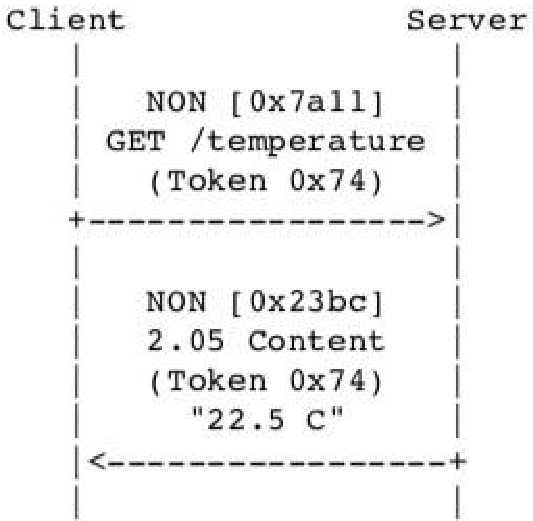
\includegraphics[height=.5\textwidth]{fig4.pdf}
    \caption
    {\label{fig:fig4} Requisição e resposta utilizando mensagens não confirmáveis.} \cite{rfc7252}
\end{figure}

A arquitetura REST, assim como no protocolo HTTP\cite{rfc2616}, foi utilizada na projetização do protocolo CoAP.
Como ambos compartilham da mesma arquitetura, realizar o mapeamento de HTTP para CoAP e vice-versa é bastante simples.
Para realizar tal mapeamento basta utilizarmos o \textit{cross-proxy}, definido na sessão 10 da própria RFC-7252\cite{rfc7252},
que converte o método ou tipo de resposta, tipo de mídia e opções para os valores HTTP correspondentes.

Além de modelo de comunicação cliente/servidor e arquitetura REST, o CoAP também dispõem de outros princípios comuns ao HTTP e que são conceitos padrão na web
como suporte a URIs\cite{rfc3986} e tipos de mídia da Internet(MIME)\cite{rfc2046}.

Entre o HTTP e CoaP nem tudo são semelhanças, pois, obviamente, este possui particularidades para que consiga atender aos requisitos no qual se propõe a resolver.
Entre as diferenças está a troca de mensagens assíncronas utilizando transporte orientado a datagramas, como UDP.
Apesar de, naturalmente, o protocolo UDP não prover confiabilidade, no CoAP é possível definir que as mensagens possuam tal aspecto.

\textit{Constrained RESTful Environments (CoRE) Link Format}, que será abordado na sessão a seguir, possibilidade de envio de solicitações multicast e unicast, \textit{service discovery}, cabeçalho com baixa sobrecarga de dados e segurança na forma de DTLS\cite{rfc6347}
estão entre as principais caracteristicas do protocolo de aplicação restrita, CoAP.



\section{Constrained RESTful Environments (CoRE) Link Format}

Segundo a RFC-6690, a finalidade deste especificação é realizar REST em nodos com recursos limitados sendo importante em aplicações maquina-a-maquina\cite{rfc6690}.
Em aplicação deste tipo é muito importante que as configurações não dependam de interação de humanos.

A principal função desta especificação é fornecer identificadores para os recursos hospedados no servidor complementado por atributos sobre estes recursos....




De forma análoga ao HTTP  e o HTTPS, o protocolo CoAP provê suporte aos esquemas do tipo \textit{coap} e \textit{coaps}, este utilizando segurança DTLS.
Estes esquemas são utilizados para identificar e localizar os recursos coap na rede.
Portanto, servidores coap ficam aguardando por requisições que utilizem tal esquema.

A definição sintática, segundo Backus-Naur Form RFC-5234\cite{rfc5234},  do  CoAP-URI está definida abaixo:

\begin{verbatim}
    CoAP-URI = "coap:" "//" host [ ":" port ] path-abempty [ "?" query ]
\end{verbatim}





O esquema CoAP-URI suporta o prefixo \textit{/.well-known/} , definido na RFC-5785\cite{rfc5785}.
Este prefixo é utilizado para que o servidor exponha suas políticas e recursos disponíveis.

O exemplo abaixa demostra um fluxo de requisição e resposta utilizando o prefixo \textit{/.well-known/}.

\begin{verbatim}
    REQ: GET coap://example.net/.well-known/core
\end{verbatim}

\begin{verbatim}
    RES: 2.05 Content
    </sensors/temp>;if="sensor",
    </sensors/light>;if="sensor"
\end{verbatim}

Notamos, então, que o servidor nomeado example.net possui os recursos \textit{temp} e \textit{light} disponíveis para serem utilizados através do protocolo coap.

\section{Trabalhos Relacionados}

% iotivity

Spencer Lewson implementou um protocolo em nível de aplicação \cite{tanenbaum2011redes} capaz de realizar a comunicação entre nodos sob computação em névoa.
A especificação do protocolo e um \textit{middleware}, capaz de realizar o gerenciamento dos recursos dos dispositivos, são os principais componentes deste trabalho \cite{Spencer:2015}.

Sua implementação requer que haja um ponto central de comunicação entre os nodos, uma vez que a conectividade entre eles ocorre via \textit{Bluetooth LE}.
A existência desse ponto justifica-se pelas regras de implementação do \textit{Bluetooth LE}, na qual descreve dispositivos de duas naturezas: centrais e periféricos.
Dispositivos centrais são responsáveis por descobrir dispositivos periféricos que estão interessados em criar conexão.
Portanto, a característica do \textit{Bluetooth LE} faz com que a topologia de rede e a arquitetura do projeto não seja distribuída \cite{Spencer:2015}.





